\section{Introduction}
\label{sec:intro}
% dialogue -> fairness in dialogues => dialogue understanding tasks
%Dialogues as the most natural way for information exchanges has gained great attention and its research directions can be divided into two categories. One is open-ended dialogue systems~\cite{gu2021dialogbert,xu2021learning} which aims at generating or selecting appropriate responses to fulfill the users' needs. The other is dialogue understanding tasks which helps to quickly digest information and returns the expected output given the whole dialogue. 

%With the prosperous of fine-tuning with pre-trained language models, dramatic improvements have achieved on a range of dialogue tasks, pushing their implementation in practice. 
%\JQ{response generation not applicable; static dialogue generation}
%\JQ{sensitivity of speaker names ia a part of fairness issue ?}
The safety and fairness issue of generations from 
dialogue models is a crucial concern in real applications. 
Previous work focuses on response generation from open-ended dialogue systems~\cite{xu2020recipes, henderson2018ethical}, such as offensive contents~\cite{baheti2021just}, gender bias~\cite{liu2020does,dinan2020queens} and other discriminated behavior~\cite{sheng2021revealing,smith2021hi}. For other text generation tasks where the whole dialogue is provided and the 
output shouldn't go beyond the dialogue, such as dialogue summarization~\cite{gliwa2019samsum} and dialogue reading comprehension~\cite{li2020molweni},
the fairness issue is still unexplored. %\JQ{more example tasks}

% leaving the fairness of close-style dialogue understanding tasks unexplored.

\begin{figure}[th]
	\centering
	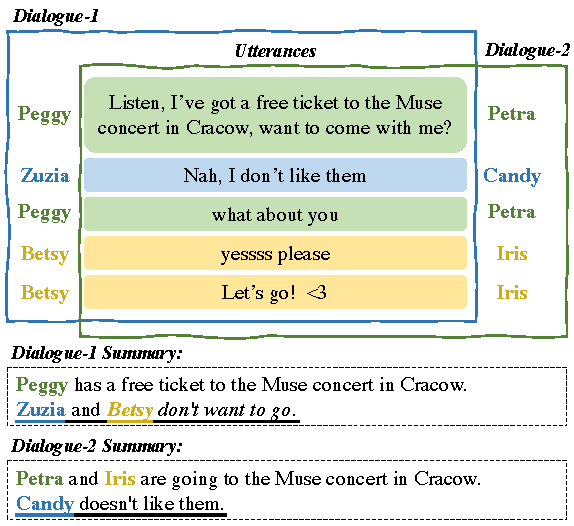
\includegraphics[width=0.9\columnwidth]{example-prev.pdf}
	\caption{Two instances of an example from the SAMSum dataset, each
with a different set of names. Two different summaries are generated by BART. 
Different colors indicate different speakers. \underline{divergent contents} are underlined and \textit{incorrect contents} are italicized.} %in the summaries.}
%\underline{Divergent contents} are underlined in the generated summaries.}
	\label{fig:example}
\end{figure}

% dialogue understanding tasks, characteristics  with example
%Representative dialogue understanding tasks includes dialogue summarization~\cite{lin2022other,zhong2022dialoglm}, reading comprehension~\cite{sun2019dream,li2020molweni}, and etc. 
In these tasks, the input dialogues are self-contained, and the names of the speakers
do not carry any connotation from outside of the dialogue. 
Therefore,
changing the speaker names consistently in a dialogue should not affect the 
meanings of the dialogue and the desired outputs.
This contrasts with response generation, where the dialogue is in progress and the output is expected to be different in styles or contents for various speakers.
Taking dialogue summarization~\cite{gliwa2019samsum,chen2021dialogsum} as an example for text generation from dialogues, it focuses on
%An example for text generation from dialogues is dialogue summarization tasks in \citet{gliwa2019samsum} and \citet{chen2021dialogsum}, focusing on
generating concise ``who-did-what'' summaries in the third person.
In Fig.~\ref{fig:example},
%Taking the dialogues in 
%Fig.~\ref{fig:example} as an example, 
the two dialogues are identical except for the speaker names. 
The two summaries are expected to be the same modulo 
the speaker names. 
%In conclusion, speaker name insensitivity is an inherent and obvious characteristic of dialogue understanding.

% robustness of language model
Unfortunately, models nowadays, following the pretrain-finetune paradigm, 
are sensitive to trivial changes, which has been verified in other tasks. 
In relation extraction, spurious correlations between entity mentions and 
relations lead to entity bias~\cite{zhang2018graph,zhang-etal-2017-position,wang-etal-2022-rely}. 
%Some work~\cite{zhang2018graph,zhang-etal-2017-position} proposes to 
%prevent it by masking entities during fine-tuning. 
%\citet{wang-etal-2022-rely} debiases the models by removing the 
%counterfactual predictions based on causal inference. 
Other similar work includes the analysis of robustness by entity 
renaming for machine reading comprehension models on narrative 
texts~\cite{yan2022robustness} and name biases in machine translation 
with inflected languages~\cite{wang2022measuring}, like German. 
Besides, \citet{shwartz2020you} claims that pre-trained language models do not treat given names as interchangeable or anonymous, showing unfairness in reading comprehension.% by switching names with pre-defined templates. % with span-based or classification models 
%\JQ{add ~\cite{shwartz2020you} Pre-trained LMs do not treat given names as interchangeable or anonymous: This has not only implications for the quality and accuracy of systems that employ these LMs, but also for the fairness of those systems.}

% sensitivity of PrLMs in dialogue understanding tasks
Obviously, dialogue understanding models are sensitive to speaker names 
according to Fig.~\ref{fig:example} as well. 
The model tends to generate different information 
given different speaker names, such as ``don't want to go'' and 
``doesn't like them''.
Incorrect content, 
``... Betsy don't want to go'', is generated with the first group of speakers, 
while not with the other group. 
%``Ashley is on her way'' and 
%``Derek will bring the dog''.  
According to our pilot experiment with the vanilla BART fine-tuned on SAMSum, around 74.00\% of generations are changed by switching speaker names and 69.82\% among them are due to distinct contents.
Such uneven performances %can lead to differences on information allocation and 
create unfairness among 
different speakers, especially in the aspect of information allocation. 
The model may also catch latent properties 
in names~\cite{romanov2019s} and lead to discrimination, %against specific groups, 
raising the importance of research on the sensitivity on speaker names.
%Different from named entities, 
%\KZ{Don't understand this: 
%speakers in these tasks are more isolated 
%from the dialogue contents and have closer connections to users in real applications}, 


Previous work has also mentioned this problem. Different data pre-processing approaches are adopted during the construction of datasets to avoid using speaker names, such as ``A'' or ``B'' in \citet{li2017dailydialog}. \citet{khalifa2021bag} replace speaker names with more common and frequent names that the model may have seen during pre-training. Data augmentation by changing speaker names is adopted by \citet{liu2021controllable}.
However, all of them only attempted to attack this problem 
subjectively, without quantitive analysis and fair comparisons. %these works

% approach classification / our approach
In this work, we systematically analyze speaker name sensitivity in text generation from dialogues. We define the speaker name sensitivity and divide the approaches 
into offline and online ones. 
Then, we propose two novel insensitivity losses, helping to reduce attention and hidden state distances of the same dialogue with different speaker names for transformer-based models during fine-tuning. These losses can be used in both kinds of approaches.
Results on several tasks show that
%online approach which replaces names with frequent ones achieves the best generation performance, and coupled with data augmentation, it provides
%the best fairness among all baselines.
our losses reduce the sensitivity and get better generations. %on task-specific metrics. %, achieving the state-of-the-art performance.
%\KZ{I'm a little confused reading the above two sentences. Which one is better,
%the freq or our ins loss?}
% contributions
In summary, our contributions are:
\begin{itemize}
	\item We are the first to investigate the speaker name sensitivity 
in text generation from dialogues (Sec.~\ref{sec:problem}) with all of the codes and results open-sourced at \url{https://github.com/JiaQiSJTU/SpeakerNameSensitivity}.% and quantify the performance sensitivity for further analysis
	\item We introduce two novel insensitivity losses as auxiliary training objectives for reducing sensitivity during fine-tuning (Sec.~\ref{sec:approach}).
	\item Experiments on different tasks provide a benchmark with comprehensive analysis on speaker name sensitivity, and show  state-of-the-art performances of our approach
%stronger overall performance with lower speaker name sensitivity 
(Sec.~\ref{sec:results}).
\end{itemize}
